\documentclass[../main.tex]{subfiles}

\begin{document}
\begin{example}
    Il frame $(\mathbb{N},R)$, dove $R = \{(n,n+1) : n \in \mathbb{N}\} \subseteq \mathbb{N} \times \mathbb{N}$ è rappresentato dal seguente grafo diretto:
    \begin{center}
        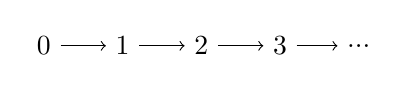
\begin{tikzpicture}[->]
            \node (0) {0};
            \node (1) [right of=0] {1};
            \node (2) [right of=1] {2};
            \node (3) [right of=2] {3};
            \node (4) [right of=3] {...};

            \path
            (0) edge node {} (1)
            (1) edge node {} (2)
            (2) edge node {} (3)
            (3) edge node {} (4);
        \end{tikzpicture}
    \end{center}
\end{example}
\begin{example}
    Il frame $(S,R)$ dove $S = \{2,3,4,5,6\}$ e $R=\{(x,y) \in S \times S : x \text{ divide } y \}$ è rappresentato dal seguente grafo diretto:
    \begin{center}
        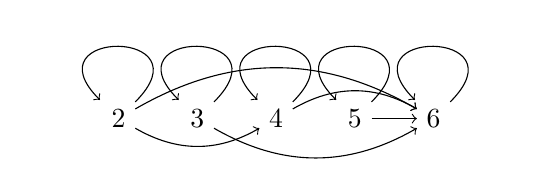
\begin{tikzpicture}[->]
            \node (2) {2};
            \node (3) [right of=2] {3};
            \node (4) [right of=3] {4};
            \node (5) [right of=4] {5};
            \node (6) [right of=5] {6};

            \path
            (2) edge[loop] node {} (2)
            (2) edge[bend right] node {} (4)
            (2) edge[bend left] node {} (6)
            (3) edge[loop] node {} (3)
            (3) edge[bend right] node {} (6)
            (4) edge[loop] node {} (4)
            (4) edge[bend left] node {} (6)
            (5) edge[loop] node {} (5)
            (5) edge node {} (6)
            (6) edge[loop] node {} (6);
        \end{tikzpicture}
    \end{center}
\end{example}
\begin{example}
    Il frame $(\{1,2,3\}, R)$ dove $R = \{(x,y) \in \{1,2,3\} \times \{1,2,3\} : y=f(x)\}$ essedo $f : \{1,2,3\} \rightarrow \{1,2,3\}$ la funzione definita da $f(1) = 2, f(2) = 3, f(3) = 1$ è
    \begin{center}
        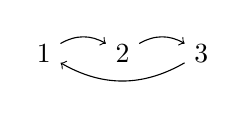
\begin{tikzpicture}[->]
            \node (1) {1};
            \node (2) [right of=1] {2};
            \node (3) [right of=2] {3};

            \path
            (1) edge[bend left] node {} (2)
            (2) edge[bend left] node {} (3)
            (3) edge[bend left] node {} (1);
        \end{tikzpicture}
    \end{center}
\end{example}
\begin{definition}[Modello]
    Un \textbf{modello} su un frame $(S,R)$ è una terna $(S,R,V)$ dove $V : Var \rightarrow \mathcal{P}(S) $, ci dice in quali mondi le variabili valgono 1 è detta \textbf{funzione di valutazione}.
\end{definition}
\begin{definition}
    Una formula $F$ si dice \textbf{Vera in un mondo x del modello M} e scriviamo $M \vDash_x F$ se e solo se:
    \begin{enumerate}
        \item \underline{F è una variabile}: $M \vDash_x F$ significa che $x \in V(F)$
        \item \underline{ F è $\neg y$ e $y$ è una variabile}: $M \vDash_x F$ significa che $x \notin V(y)$
        \item \underline{F è del tipo $\neg G$}, dove $G$ è una formula: $M \vDash_x F$ significa che $M \nvDash_x G$
        \item \underline{F è del tipo $G_1 \land G_2$}: $M \vdash_x F$ significa che $M \vdash_x G_1$ e $M \vDash_x G_2$
        \item \underline{F è del tipo $G_1 \lor G_2$}: $M \vdash_x F$ significa che $M \vdash_x G_1$ o $M \vDash_x G_2$
        \item \underline{F è del tipo $\Box G$}: $M \vDash_x F$ significa che $M \vDash_y G$, per ogni $y \in S : (x,y) \in R$, ossia per ogni mondo y raggiungibile da $x$.
        \item \underline{F è del tipo $\Diamond G$}: $M \vDash_x F$ significa che $M \vDash_y G$ per qualche $y \in S : (x,y) \in R$, ossia per almeno un mondo raggiungibile da $x$.
    \end{enumerate}
\end{definition}
\begin{definition}[Soddisfacibilità]
    Una formula $F$ è \textbf{soddisfacibile} se esiste un modello $M = (S, R, V)$ e un mondo $x \in S$, tali che $M \vDash_x F$.
\end{definition}
\begin{theorem}
    Se una formula modale $F$ è soddisfacibile, allora è soddisfacibile in una struttura di Kripke $(S,R)$ tale che $|S| \leq 2^{|F|}$, $|F| = $"lunghezza di F".

    Quindi il problema di soddisfacibilità di una formula modale è decidibile.
\end{theorem}

Se come frame prendiamo $({0},R)$ dove $R \subseteq S \times S = \{(0,0)\}$ è quindi $S$ stesso, una funzione di valutazione è $V : Var \rightarrow \mathcal{P}(S) = \{\emptyset, \{0\}\} \simeq \{0,1\}$.

In questo modo i connettivi modali diventano superflui e ritroviamo la logica modale che abbiamo già studiato.

La veritò di una formula del linguaggio della logica modale dipenderà quindi dal frame scelto, in particolare dalla relazione $R$.

Ad esempio nella logica della necessità vogliamo che sia sempre vera la formula
\begin{equation*}
    \Box x \implies x \qquad \text{"è necessaria che $x$, allora $x$"}
\end{equation*}
Nella logica deontica la stessa formula la leggiamo "è obbligatorio che $x$, allora $x$" e non vogliamo che questa affermazione sia sempre vera.

Perchè sia sempre vera la formula $\Box x \implies x$, la relazione $R$ del frame deve essere riflessiva, ossia $(y,y) \in R \forall y \in S$.

Infatti, se $R$ non fosse riflessiva ci sarebbe un mondo $y \in S$ tale che $(y,y) \notin R$.

Sia $Z = V(x), Z \subseteq S,$ tale che $y \notin Z$ (cioè x è falsa nel mondo y).

Sia $Z \supseteq \{z \in S : (y,z) \in R\}$ cioè x sia vera in tutti i mondi accessibili da y.

Allora se $M = (S, R, V), M \vDash_y \Box x$ ma $M \nvDash_y x$.

Nella logica deontica, dove non vogliamo che sia sempre vera la formula $\Box x \implies x$, non prenderemo una relazione riflessiva.
\begin{definition}
    Una formula $F$ si dice \textbf{vera in un modello M}, scritto \textbf{$M \vDash F$}, se $M \vDash_x F, \forall x \in S$, ossia se è vera in tutti i mondi di $S$.
\end{definition}
\begin{definition}
    Una formula si dice \textbf{valida in un frame $(S,R)$}, scritto $(S,R) \vDash F$, se è vera in tutti i modelli costruiti su $(S,R)$.
\end{definition}
\begin{example}
    La formula $\Box x \implies x$ è valida solo nel frame $(S,R)$ in cui $R$ è riflessiva.
\end{example}
\begin{definition}[Formula Valida]
    Una formula $F$ è \textbf{valida} se e solo se è valida su ogni frame, e scriviamo $\vDash F$
\end{definition}
\begin{definition}[Schema di Formule]
    Uno \textbf{schema di formule} è una collezione di formule aventi tutte la stessa forma sintattica.

    Ad esempio, con lo schema $\Box x \implies x$ si intendono tutte le forume di questa forma, come $\Box x \implies x$, $x$ variabile, o $\Box (\neg \Diamond \neg x) \implies \neg \Diamond \neg x$.
\end{definition}
Le tautologie della logica proposizionale sono valide su ogni frame.

Vediamo ora che lo schema di formule $\Box (A \implies B) \implies (\Box A \implies \Box B)$ \\
è valido su ogni frame.

Sia $w \in S$ un mondo e M un modello su un frame $(S,R)$.

Sia $M \vDash_w \Box (A \implies B)$ e $M \vDash_w \Box A$. (dobbiamo solo controllare che quando $\Box ( A \implies B )$ è vera, allora se è vera $\Box A$, è vera $\Box B$).

$M \vDash_w \Box (A \implies B)$ significa che $M \vDash_v A \implies B, \forall v \in S t.c. (w,v) \in R$.

$M \vDash_w \Box A$ significa che $M \vDash_v A, \forall v \in S t.c. (w,v) \in R$.

Dunque $M \vDash_v B, \forall v \in S t.c. (w,v) \in R$, ossia $M \vDash_w \Box B$.

Abbiamo dimostrato che
\begin{equation*}
    \vDash \Box (A \implies B) \implies (\Box A \implies \Box B)
\end{equation*}
Chiameremo $K$ tale schema.

Mostriamo che i seguenti schemi sono validi:
\begin{enumerate}
    \item $\Box (A \land B) \iff (\Box A \land \Box B)$
    \item $\Diamond (A \lor B) \iff (\Diamond A \lor \Diamond B)$
    \item $\Box (A \implies B) \implies (\Diamond A \implies \Diamond B)$
    \item $\Diamond (A \implies B) \implies (\Box A \implies \Diamond B)$
\end{enumerate}
\begin{enumerate}
    \item $M \vDash_w \Box (A \land B)$ se e solo se $M \vDash_v A \land B, \forall v \in S t.c. (w,v) \in R$,\\
          se e solo se $M \vDash_v A \text{ e } M \vDash_v B \forall v \in S t.c. (w,v) \in R$,\\
          se e solo se $M \vDash_w \Box A$ e $M \vDash_w \Box B$,\\
          se e solo se $M \vDash_w (\Box A \land \Box B)$, dove M è un modello su un frame $(S,R)$ e $w \in S$
    \item $M \vDash_w \Diamond (A \lor B)$ se e solo se $M \vDash_v A \lor B, \exists v \in S t.c. (w,v) \in R$,\\
          se e solo se $M \vDash_v A \text{ o } M \vDash_v B \exists v \in S t.c. (w,v) \in R$,\\
          se e solo se $M \vDash_w \Diamond A \text{ o } M \vDash_w \Diamond B$,\\
          se e solo se $M \vDash_w (\Diamond A \lor \Diamond B)$, dove M è un modello su un frame $(S,R)$ e $w \in S$
    \item $M \vDash_w \Box (A \implies B)$ e $M \vDash_w \Diamond A$ implicano che $M \vDash_v (A \implies B), \forall v \in S t.c. (w,v) \in R$,\\
          e $M \vDash_v A, \exists v \in S t.c. (w,v) \in R$.\\
          Quindi $M \vDash_v B, \exists  v \in S$ t.c. $(w,v) \in R$,\\
          ossia $M \vDash_w \Diamond B$, dove $M$ è un modello su un frame $(S,R)$ e $w \in S$
    \item $M \vDash_w \Diamond (A \implies B)$ e $M \vDash_w \Box A$ implicano che $M \vDash_v (A \implies B), \exists v \in S t.c. (w,v) \in R$, e $M \vDash_v A, \forall v \in S t.c. (w,v) \in R$.

          Quindi $M \vDash_v B, \exists v \in S t.c. (w,v) \in R$, ossia $M \vDash_w \Diamond B$, dove $M$ è un modello su un frame $(S,R)$ e $w \in S$
\end{enumerate}
Abbiamo già mostrato che se M è un modello su un frame $(S,R)$ con $R$ non riflessiva, allora $\Box x \implies x$ non è vera nel modello $M$. Quindi la formula $\Box x \implies x$ non è valida.
\begin{equation*}
    \nvDash \Box x \implies x
\end{equation*}
Mostiamo che i seguenti schemi di fromule non sono validi:
\begin{enumerate}
    \item $\Diamond A \implies \Box A$
    \item $\Box A \implies A$ (già visto)
    \item $\Box A \implies \Box \Box A$
    \item $\Box (A \implies B) \implies (\Box A \implies \Diamond B)$
    \item $\Box (\Box A \implies B) \lor \Box (\Box B \implies A)$
    \item $\Box (A \lor B) \implies (\Box A \lor \Box B)$
    \item $\Box(\Box A \implies A) \implies \Box A$
\end{enumerate}
\begin{enumerate}
    \item \begin{equation*}
              \begin{tikzpicture}[->]
                  \node (1) {1};
                  \node (2) [right of=1] {2};
                  \path
                  (1) edge[loop] node {} (1)
                  (1) edge node {} (2);
              \end{tikzpicture}
              \qquad
              M = (\{1,2\},\{(1,2),(1,1)\}, V)
          \end{equation*}

          $V(x) = 2 $ (ossia la formiula x è vera solo nel mondo 2) quindi $M \vDash_! \Diamond x$ e $M \nvDash_1 \Box x$, ossia $M \nvDash_1 (\Diamond x \implies \Box x)$
    \item già visto.
    \item \begin{equation*}
              \begin{tikzpicture}[->]
                  \node (1) {1};
                  \node (2) [right of=1] {2};
                  \node (3) [right of=2] {3};
                  \path
                  (1) edge node {} (2)
                  (2) edge node {} (3);
              \end{tikzpicture}
              \qquad
              M = (\{1,2,3\},\{(1,2),(2,3)\}, V)
          \end{equation*}

          $V(x) = \{2\}$ Quindi $M \vDash_1 \Box x$.

          Abbiamo che $M \vDash_1 \Box \Box x$ se e solo se $M \vDash_2 \Box x$, se e solo se $M \vDash_3 x$, ma $M \nvDash_3 x$, quindi $M \nvDash_1 \Box \Box x$
    \item \begin{equation*}
              \begin{tikzpicture}[->]
                  \node (1) {1};
                  \node (2) [right of=1] {2};
                  \path
                  (1) edge node {} (2);
              \end{tikzpicture}
              \qquad
              M = (\{1,2\}, V)
          \end{equation*}

          $V(x) = \{1\}$ $M \vDash_2 \Box (A \implies B)$, $M \vDash_2 \Box A$, ma $M \nvDash_2 \Diamond B$, perchè non esiste $v \in \{1,2\} t.c M \vDash_v , (2,v) \in R$
    \item prendiamo $A = B = x$ nel frame
          \begin{equation*}
              \begin{tikzpicture}[->]
                  \node (1) {1};
                  \node (2) [right of=1] {2};
                  \node (3) [right of=2] {3};
                  \path
                  (1) edge node {} (2)
                  (2) edge node {} (3);
              \end{tikzpicture}
              \qquad
              M = (\{1,2,3\},\{(1,2),(2,3)\}, V)
          \end{equation*}

          $V(x) = \{3\}$, si ha $M \vDash_1 \Box (\Box x \implies x)$ se e solo se $M \vDash_2 \Box x \implies x$, se e solo se $M \vDash_3 x$ e $M \nvDash_2 x$, ma $M \nvDash_2 \Box x$, quindi $M \nvDash_1 \Box (\Box x \implies x)$
    \item \begin{equation*}
              \begin{tikzpicture}[->]
                  \node (1) {1};
                  \node (2) [right of=1] {2};
                  \path
                  (1) edge[loop] node {} (1)
                  (1) edge node {} (2);
              \end{tikzpicture}
              \qquad
              M = (\{1,2\},\{(1,2),(1,1),\}, V)
          \end{equation*}

          $V(x) = \{1\}, V(y) = \{2\}$ $M \vDash_1 \Box (x \lor y)$ se e solo se $M \nvDash_1 (x \lor y)$ e $M \nvDash_2 (x \lor y)$.

          Quindi abbiamo che $M \nvDash_1 \Box (x \lor y)$.

          Invece $M \vDash_1 (\Box x \lor \Box y)$ se e solo se $M \vDash_1 x$ e $M \vDash_2 x$ o $M \vDash_1 y$ e $M \vDash_2 y$, Dunque $M \nvDash_1 (\Box x \lor \Box y)$
    \item \begin{equation*}
              \begin{tikzpicture}[->]
                  \node (1) {1};
                  \node (2) [right of=1] {2};
                  \node (3) [right of=2] {3};
                  \path
                  (1) edge[loop] node {} (1)
                  (1) edge node {} (2)
                  (2) edge node {} (3);
              \end{tikzpicture}
              \qquad
              M = (\{1,2,3\},\{(1,2),(2,3)\}, V)
          \end{equation*}

          $V(x) = \{2,3\}$ $M \vDash_1 \Box (\Box x \implies x)$ se e solo se $M \vDash_1 (\Box x \implies x)$ e $M \vDash_2 (\Box x \implies x)$, che sono entrambe vere, quindi $M \vDash_1 \Box (\Box x \implies x)$ invece $M \nvDash_1 \Box x$ perchè $M \nvDash_1 x$.
\end{enumerate}

\section{Corrispondenza e Non Esprimibilità}
\begin{definition}
    diciamo che un frame $(S,R)$ gode di una certa proprietà se ne gode la relazione $R$.

    In molti casi una proprietà di un frame equivale alla validità di uno schema di formule modali nei frame con quella proprietà.
\end{definition}
\begin{theorem}
    Lo schema $\Box A \implies A$ è valido in un frame $(S,R)$ se e solo se $R$ è riflessiva.
\end{theorem}
\begin{proof}
    Già visto.
\end{proof}
\begin{theorem}
    Lo schema $ A \implies \Box \Diamond A$ è valido in un frame $(S,R)$ se e solo se $R$ è simmetrica.
\end{theorem}
\begin{proof}
    Sia $R$ simmetrica, ossia $(x,y) \in R \implies (y,x) \in R$.

    Sia $M \vDash_w A$ e $(w,v) \in R$. Dunque $(v,w) \in R$ e $M \vDash_v \Diamond A \forall v \in S$ t.c. $(w,v) \in R$, ossia $M \vDash_w \Box \Diamond A$.

    Adesso assumiamo che lo schema $A \implies \Box \Diamond A $ sia valido in $(S,R)$.

    Sia x una variabile e $V(x) = \{s\}$;

    sia $t \in S$ t.c. $(s,t) \in R$. Quindi $M \vDash_s x$.

    Dalla validità dello schema segue allora che $M \vDash_s \Box \Diamond x$, da cui $M \vDash_t \Diamond x$.

    Quindi esiste $r \in S$ t.c. $(t,r) \in R e M \vDash_r x$, ossia $r = s$
\end{proof}
\begin{theorem}
    Lo schema $\Box A \implies \Box \Box A$ è valido in un frame $(S,R)$ se e solo se R è transitiva.
\end{theorem}
\begin{proof}
    Sia $R$ transitiva, ossia $(x,y) \in R, (y,z) \in R \implies (x,z) \in R$.

    Sia $M \vDash_w \Box A$, ossia $M \vDash_v A \forall v \in S$ t.c. $(w,v) \in R$.

    Sia $u \in S$ t.c. $(v,u) \in R$, con $(w,v) \in R$.

    Allora $(w,u) \in R$ e quindi $M \vDash_v \Box A, \forall v \in S$ t.c. $(w,v) \in R$, ossia $M \vDash_w \Box \Box A$.

    Assumiamo adesso che sia valido lo schema $\Box A \implies \Box \Box A$ su un frame $(S,R)$.

    Sia $x$ una variabile, $s \in S$ e $V(x) = \{w \in S : (s,w) \in R\}$.

    Allora $M \vDash_s \Box x$ e quindi per la validità dello schema, $M \vDash_s \Box \Box x $, da cui $M \vDash_t \Box x \forall t \in S$ t.c. $(s,t) \in R$, ossia $M \vDash_r x \forall r \in S$ t.c. $(t,r) \in R$, $(s,t) \in R$.

    Da ciò segue che $r \in V(x)$ ossia $(s,t) \in R$ e $(t,r) \in R \implies (s,r) \in R$\\
\end{proof}
Adesso vediamo che ci sono anche proprietà dei frame non esprimibili in termini di validità di schemi di formule modali.

\section{Morfismi di modelli}
\begin{definition}[Morfismo di Frame]
    Siano $(S_1, R_1)$ e $(S_2, R_2)$ due frame. una funzione $f : S_1 \rightarrow S_2$ è un \textbf{morfismo di frame} se:
    \begin{equation*}
        (x,y)\in R_1 \implies (f(x), f(y)) \in R_2 \qquad \forall x,y \in S_1
    \end{equation*}
\end{definition}
\begin{example}
    Siano $(\mathbb{N}, R_1)$ e $(\mathbb{N}, R_2)$ i frame tali che
    \begin{equation*}
        R_1 = R_2 = \{(x,y) \in \mathbb{N} \times \mathbb{N} : x < y\}
    \end{equation*}
    allora la funzione
    \begin{align*}
        f : \; \mathbb{N} & \rightarrow \mathbb{N} \\
        n                 & \mapsto n^2
    \end{align*}
    è un morfismo di frame.
\end{example}
\end{document}